%%%%%%%%%%%%%%%%%%%%% Appendix A %%%%%%%%%%%%%%%%%%%%%%%%%%%%%%%%%%%
% The Economic Case for Trustworthy AI:
% A Risk-Adjusted Value Framework for Architects and Decision-Makers
%%%%%%%%%%%%%%%%%%%%%%%%%%%%%%%%%%%%%%%%%%%%%%%%%%%%%%%%%%%%%%%%%%%%

% ------------------------------------------------------------------
%  Colour definitions
% ------------------------------------------------------------------
\definecolor{losscol}{RGB}{220,  53,  53}
\definecolor{gaincol}{RGB}{ 56, 168,  80}
\definecolor{costcol}{RGB}{255, 180,   0}
\definecolor{casebg} {RGB}{245, 247, 250}
\definecolor{formulabg}{RGB}{235, 243, 255}

% ------------------------------------------------------------------
%  tcolorbox styles
% ------------------------------------------------------------------
\tcbset{
  casebox/.style={
    enhanced, colback=casebg,
    colframe=gray!55, fonttitle=\bfseries\small,
    left=8pt, right=8pt, top=6pt, bottom=6pt,
    breakable
  },
  formulabox/.style={
    enhanced, colback=formulabg,
    colframe=blue!55!black, fonttitle=\bfseries\small,
    left=8pt, right=8pt, top=6pt, bottom=6pt,
    breakable
  }
}

% ==================================================================
\chapter{The Economic Case for Trustworthy AI: A Risk-Adjusted
         Value Framework}
\label{app:roi-of-trust}
% ==================================================================

\begin{quote}
\textit{``Security is always excessive until the day it is not
enough.''
\hfill ---William~O.~Douglas \\[6pt]
``The CFO does not care about zero-knowledge proofs.
The CFO cares about what happens when you do not have one.''}
\end{quote}

\section*{Purpose and Audience}
\label{sec:app-purpose}

Every chapter of this book has addressed the \emph{technical}
case for Trustworthy AI: why Differential Privacy is mathematically
superior to k-anonymity, why ZK-proofs close the verifiability
gap, why TEEs protect data in use.
What the preceding chapters have not addressed is the question
that determines whether any of those technologies ever gets
funded: \emph{what is it worth?}

This appendix is written for two audiences simultaneously.
The \textbf{architect} who must translate technical risk into
financial language for a budget conversation.
And the \textbf{executive} --- Chief Financial Officer,
Chief Risk Officer, or Board member --- who must decide how
much to spend on capabilities that are, by design, invisible
when they work.

The framework presented here is the
\textbf{Risk-Adjusted Value (RAV) of Trust}: a structured
methodology for calculating the financial return on investment
of each layer of the Trustworthy AI Stack, grounded in the
real-world incident costs of the 2025 crisis events introduced
in Chapter~\ref{chap:vision}.

% ------------------------------------------------------------------
\section{The Invisible Feature Problem}
\label{sec:invisible-feature}
% ------------------------------------------------------------------

Trustworthy AI mechanisms share an uncomfortable economic
property: their value is most visible in the counterfactual.
A ZK-proof layer that prevents a fraudulent audit costs money
every day.
The fraud it prevents is invisible, because it never happens.

This creates a systematic \textbf{Underinvestment Trap} in
technology budgeting.
Product features that users can see and measure generate direct
revenue signals.
Trust mechanisms that users never notice generate no such signal
--- until the moment they fail, at which point the cost of
their absence arrives in a single catastrophic event.

The Underinvestment Trap is not a failure of executive
rationality.
It is a failure of \emph{information}: executives cannot
rationally invest in risks they cannot quantify.
The RAV framework is designed to close that information gap
by translating the probabilistic language of threat modelling
into the deterministic language of expected value that
financial decision-makers require.

\subsection{The Asymmetry of Trust Costs}
\label{subsec:cost-asymmetry}

The fundamental economic asymmetry of trust is expressed in
two inequalities that should appear on the first slide of
every budget presentation an architect gives:

\begin{tcolorbox}[formulabox]
\begin{equation}
  \label{eq:cost-asymmetry}
  C_{\mathrm{prevention}}
    \ll C_{\mathrm{incident}}
  \qquad \text{and} \qquad
  T_{\mathrm{prevention}}
    \ll T_{\mathrm{recovery}}
\end{equation}

where $C$ denotes financial cost and $T$ denotes calendar time.
\end{tcolorbox}

Table~\ref{tab:cost-asymmetry-evidence} quantifies this
asymmetry for the four incident classes introduced in
Chapter~\ref{chap:vision}, using published regulatory penalty
structures and industry breach-cost benchmarks.

\begin{table}[ht]
\centering
\caption{Cost asymmetry between trust mechanism investment and
  incident remediation for four 2025 incident classes.
  Prevention costs are annualised for a mid-sized Vietnamese
  enterprise (500--2{,}000 employees, \$50M--\$200M revenue).
  Incident costs are derived from the specific 2025 cases and
  scaled to the Vietnamese regulatory environment under
  Decree~13 and the AI Law (effective March 2026).}
\label{tab:cost-asymmetry-evidence}
\small
\begin{tabular}{p{2.8cm}p{2.4cm}rrr}
\hline\noalign{\smallskip}
\textbf{Incident Class}
  & \textbf{2025 Reference Case}
  & \textbf{Prevention Cost (USD/yr)}
  & \textbf{Incident Cost (USD)}
  & \textbf{Cost Ratio} \\
\noalign{\smallskip}\svhline\noalign{\smallskip}

PII Data Breach (prompt injection)
  & McHire Security Breach (2M applicants)
  & \$45K--\$120K
  & \$14.8M--\$38.2M
  & $\mathbf{123\times}$--$\mathbf{847\times}$ \\[4pt]

Deepfake Fraud
  & CEO Agent Mimicry (\$50M transfer)
  & \$28K--\$85K
  & \$50M + \$12M legal/recovery
  & $\mathbf{729\times}$--$\mathbf{2{,}214\times}$ \\[4pt]

Side-Channel Hardware Attack
  & LedgerNet TEE Breach (10k users)
  & \$60K--\$180K
  & \$8.4M--\$22.1M
  & $\mathbf{47\times}$--$\mathbf{368\times}$ \\[4pt]

Hallucination in Healthcare
  & Diagnostic Agent Miscalibration
  & \$35K--\$95K
  & \$6.2M--\$31.5M (liability + recall)
  & $\mathbf{65\times}$--$\mathbf{900\times}$ \\

\noalign{\smallskip}\hline\noalign{\smallskip}
\end{tabular}
\end{table}

The cost ratios in Table~\ref{tab:cost-asymmetry-evidence}
range from $47\times$ to over $2{,}000\times$.
Even at the low end of this range, the expected-value case for
trust investment is overwhelming --- provided the probability
of an incident is non-negligible.
Section~\ref{sec:rav-framework} formalises this calculation.

% ------------------------------------------------------------------
\section{The 2025 Incident Taxonomy: A Financial Autopsy}
\label{sec:incident-taxonomy}
% ------------------------------------------------------------------

Before introducing the RAV formula, we perform a structured
financial autopsy of the four 2025 reference incidents.
Each autopsy disaggregates total incident cost into five
cost categories that correspond directly to the technical
failures the Trustworthy AI Stack is designed to prevent.

\begin{tcolorbox}[casebox,
  title={Financial Autopsy 1: The McHire Security Breach}]

\textbf{Technical failure:} Absent prompt-injection guardrails
and insufficient PII isolation in an autonomous recruitment agent.

\textbf{Disclosed facts:} 2,000,000 applicant records exfiltrated.
Agent manipulated via indirect prompt injection to leak data to
an external endpoint over 11 days before detection.

\medskip
\begin{tabular}{@{}lrr@{}}
\hline\noalign{\smallskip}
\textbf{Cost Category} & \textbf{USD (low)} & \textbf{USD (high)} \\
\noalign{\smallskip}\svhline\noalign{\smallskip}
Regulatory fines (Decree~13: up to 5\% revenue) & \$2.5M & \$8.0M \\
Legal settlement (class action, 2M claimants) & \$4.2M & \$14.0M \\
Incident response \& forensics & \$0.8M & \$2.4M \\
Reputational damage (revenue loss, 12 months) & \$5.1M & \$9.8M \\
System remediation \& re-audit & \$2.2M & \$4.0M \\
\noalign{\smallskip}\hline\noalign{\smallskip}
\textbf{Total} & \textbf{\$14.8M} & \textbf{\$38.2M} \\
\noalign{\smallskip}\hline\noalign{\smallskip}
\textbf{Prevention cost (input guardrails + DP)} & \$45K & \$120K \\
\textbf{Cost ratio} & $\mathbf{123\times}$ & $\mathbf{318\times}$ \\
\noalign{\smallskip}\hline\noalign{\smallskip}
\end{tabular}

\medskip
\textbf{Preventable fraction:}
The technical root causes --- missing prompt-injection detection
and absent PII masking at the output guardrail layer --- are
directly addressed by the input/output guardrail architecture
and the DP fine-tuning mechanisms described in earlier chapters.
Conservative attribution: $\geq 85\%$ of total incident cost
was preventable by a \$45K--\$120K annual investment in these
two mechanisms.
\end{tcolorbox}

\begin{tcolorbox}[casebox,
  title={Financial Autopsy 2: Deepfake-Enabled Corporate Fraud}]

\textbf{Technical failure:} No cryptographic agent identity
verification, absent ZK-audit logging, and no TEE-protected
approval pathway for high-value transactions.

\textbf{Disclosed facts:} CEO's autonomous agent mimicked via
deepfake voice and visual synthesis.
\$50M cross-border wire transfer authorised in a single
agentic action.
Fraud detected 72 hours later via manual reconciliation.

\medskip
\begin{tabular}{@{}lrr@{}}
\hline\noalign{\smallskip}
\textbf{Cost Category} & \textbf{USD (low)} & \textbf{USD (high)} \\
\noalign{\smallskip}\svhline\noalign{\smallskip}
Unrecovered transferred funds & \$32.0M & \$50.0M \\
Legal \& regulatory investigation & \$3.1M & \$7.2M \\
Executive liability \& D\&O insurance increase & \$1.8M & \$4.0M \\
Reputational \& share-price impact & \$4.4M & \$11.5M \\
System overhaul \& re-certification & \$2.8M & \$6.0M \\
\noalign{\smallskip}\hline\noalign{\smallskip}
\textbf{Total} & \textbf{\$44.1M} & \textbf{\$78.7M} \\
\noalign{\smallskip}\hline\noalign{\smallskip}
\textbf{Prevention cost (ZK-audit + TEE approval)} & \$28K & \$85K \\
\textbf{Cost ratio} & $\mathbf{519\times}$ & $\mathbf{926\times}$ \\
\noalign{\smallskip}\hline\noalign{\smallskip}
\end{tabular}

\medskip
\textbf{Preventable fraction:}
A TEE-protected, ZK-verified approval pathway for transactions
above a configurable threshold (the ``Emergency Brake'' pattern)
would have required a second authenticated principal to
authorise the transfer.
Conservative attribution: $\geq 90\%$ of total incident cost
was preventable at a \$28K--\$85K annual investment.
\end{tcolorbox}

\begin{tcolorbox}[casebox,
  title={Financial Autopsy 3: LedgerNet Side-Channel Attack}]

\textbf{Technical failure:} Sole reliance on a single TEE layer
without the defence-in-depth composition (TEE + DP + SecAgg).
Absent side-channel noise injection for timing-sensitive
memory operations.

\textbf{Disclosed facts:} \$1.2B weekly DeFi volume.
10,000 user account balances reconstructed via timing-based
side-channel attack over 48 hours.
Protocol suspended for 9 days.

\medskip
\begin{tabular}{@{}lrr@{}}
\hline\noalign{\smallskip}
\textbf{Cost Category} & \textbf{USD (low)} & \textbf{USD (high)} \\
\noalign{\smallskip}\svhline\noalign{\smallskip}
User restitution (10k accounts) & \$2.1M & \$6.8M \\
9-day protocol suspension (lost fees) & \$2.8M & \$5.4M \\
Regulatory investigation \& fines & \$1.2M & \$4.2M \\
Security audit \& hardware replacement & \$1.4M & \$3.8M \\
Reputational TVL loss (6 months) & \$0.9M & \$1.9M \\
\noalign{\smallskip}\hline\noalign{\smallskip}
\textbf{Total} & \textbf{\$8.4M} & \textbf{\$22.1M} \\
\noalign{\smallskip}\hline\noalign{\smallskip}
\textbf{Prevention cost (DP + SecAgg composition)} & \$60K & \$180K \\
\textbf{Cost ratio} & $\mathbf{140\times}$ & $\mathbf{123\times}$ \\
\noalign{\smallskip}\hline\noalign{\smallskip}
\end{tabular}

\medskip
\textbf{Preventable fraction:}
Adding Differential Privacy noise to memory-access timing
patterns and composing TEE protection with Secure Aggregation
eliminates the timing side-channel as an attack surface.
Conservative attribution: $\geq 75\%$ of total incident cost
was preventable at a \$60K--\$180K annual investment.
\end{tcolorbox}

\begin{tcolorbox}[casebox,
  title={Financial Autopsy 4: Hallucination in Healthcare}]

\textbf{Technical failure:} Missing Conformal Prediction
uncertainty quantification, absent formal verification of
safety properties, and no Trust Dashboard Uncertainty Handover
protocol (Section~\ref{subsec:trust-dashboards}).

\textbf{Disclosed facts:} Diagnostic agents producing
unrepresentative treatment recommendations for minority groups
over a 6-month period.
Detected during external audit.
Regulatory investigation triggered across three hospital networks.

\medskip
\begin{tabular}{@{}lrr@{}}
\hline\noalign{\smallskip}
\textbf{Cost Category} & \textbf{USD (low)} & \textbf{USD (high)} \\
\noalign{\smallskip}\svhline\noalign{\smallskip}
Liability settlements (affected patients) & \$2.8M & \$14.0M \\
Regulatory fines (AI Law high-risk breach) & \$1.1M & \$6.5M \\
System recall \& retraining & \$0.9M & \$3.2M \\
Clinical re-review programme & \$0.8M & \$4.8M \\
Reputational damage (contract losses) & \$0.6M & \$3.0M \\
\noalign{\smallskip}\hline\noalign{\smallskip}
\textbf{Total} & \textbf{\$6.2M} & \textbf{\$31.5M} \\
\noalign{\smallskip}\hline\noalign{\smallskip}
\textbf{Prevention cost (CP + formal verification)} & \$35K & \$95K \\
\textbf{Cost ratio} & $\mathbf{177\times}$ & $\mathbf{332\times}$ \\
\noalign{\smallskip}\hline\noalign{\smallskip}
\end{tabular}

\medskip
\textbf{Preventable fraction:}
Conformal Prediction with a calibrated uncertainty threshold
would have flagged the distribution shift for underrepresented
groups within the first two weeks of deployment.
Formal verification of the fairness property would have caught
the miscalibration pre-deployment.
Conservative attribution: $\geq 80\%$ of total incident cost
was preventable at a \$35K--\$95K annual investment.
\end{tcolorbox}

% ------------------------------------------------------------------
\section{The Risk-Adjusted Value Framework}
\label{sec:rav-framework}
% ------------------------------------------------------------------

\subsection{Core Definitions}
\label{subsec:rav-definitions}

The \textbf{Risk-Adjusted Value of Trust} $\mathrm{RAV}(m)$ for
a trust mechanism $m$ is defined as the expected reduction in
incident cost attributable to mechanism $m$, net of the annual
cost of deploying that mechanism.

We require four inputs:

\begin{description}
  \item[$L_m$ (Loss Exposure).]
    The total financial loss the organisation faces if the
    incident class that mechanism $m$ defends against
    materialises.
    Derived from the financial autopsies of
    Section~\ref{sec:incident-taxonomy} and scaled to the
    organisation's revenue, data volume, and regulatory
    jurisdiction.

  \item[$p_m$ (Incident Probability Without Mechanism).]
    The annual probability of the incident occurring in the
    absence of mechanism $m$.
    Derived from industry threat intelligence, regulatory
    incident databases, and the organisation's own historical
    data.
    For organisations with no internal data, conservative
    default values are provided in
    Table~\ref{tab:default-probabilities}.

  \item[$r_m$ (Risk Reduction Factor).]
    The fractional reduction in incident probability that
    mechanism $m$ provides.
    $r_m \in [0, 1]$, where $r_m = 1$ means the mechanism
    eliminates the risk entirely and $r_m = 0$ means it
    provides no protection.
    Conservative values from the financial autopsies are used;
    no mechanism claims $r_m = 1$.

  \item[$C_m$ (Annual Mechanism Cost).]
    The total cost of deploying and maintaining mechanism $m$
    for one year, including licensing, engineering time,
    operational overhead, and the carbon cost computed in
    Section~\ref{sec:carbon-cost-of-trust}.
\end{description}

\subsection{The RAV Formula}
\label{subsec:rav-formula}

\begin{tcolorbox}[formulabox,
  title={Definition: Risk-Adjusted Value of Trust}]
\begin{equation}
  \label{eq:rav}
  \mathrm{RAV}(m)
    = \underbrace{p_m \cdot r_m \cdot L_m}_{
        \text{Expected Loss Reduction}}
    - \underbrace{C_m}_{\text{Mechanism Cost}}
\end{equation}

A mechanism is \textbf{economically justified} if and only if
$\mathrm{RAV}(m) > 0$.
The \textbf{RAV Ratio} $\rho_m = \mathrm{RAV}(m) / C_m$
expresses the return on every dollar invested in the mechanism.
\end{tcolorbox}

\subsection{The Trust Stack RAV: Portfolio Calculation}
\label{subsec:rav-portfolio}

For a full Trustworthy AI Stack comprising mechanisms
$M = \{m_1, m_2, \ldots, m_k\}$, the portfolio RAV accounts
for the fact that mechanisms interact: deploying DP-FL reduces
the residual risk that a SecAgg layer must cover.

We model this with a \textbf{Residual Risk Chain}:

\begin{equation}
  \label{eq:residual-risk}
  p_{\mathrm{residual}}^{(k)}
    = p \cdot \prod_{i=1}^{k} (1 - r_{m_i})
\end{equation}

where $p$ is the baseline incident probability and
$r_{m_i}$ is the risk reduction factor of the $i$-th
mechanism in the stack.
The portfolio RAV is:

\begin{equation}
  \label{eq:portfolio-rav}
  \mathrm{RAV}(M)
    = L \cdot \left(
        p - p_{\mathrm{residual}}^{(k)}
      \right)
    - \sum_{i=1}^{k} C_{m_i}
\end{equation}

The \textbf{Marginal RAV} of adding mechanism $m_{k+1}$ to an
existing stack $M$ is:

\begin{equation}
  \label{eq:marginal-rav}
  \Delta\mathrm{RAV}(m_{k+1} \mid M)
    = L \cdot p_{\mathrm{residual}}^{(k)} \cdot r_{m_{k+1}}
    - C_{m_{k+1}}
\end{equation}

Equation~\eqref{eq:marginal-rav} is the formula an architect
should bring to a budget meeting.
It answers the executive's question directly:
\emph{``What does adding this specific layer to our existing
stack save us, net of what it costs?''}

% ------------------------------------------------------------------
\section{Default Probability and Cost Reference Tables}
\label{sec:default-tables}
% ------------------------------------------------------------------

\subsection{Incident Probability Defaults}
\label{subsec:default-probabilities}

Table~\ref{tab:default-probabilities} provides conservative
annual incident probability defaults for four deployment
risk tiers, derived from the NIST AI RMF 2026 incident
database, Vietnam's AI Law Conformity Assessment guidance,
and industry breach-cost benchmarks.

\begin{table}[ht]
\centering
\caption{Default annual incident probability $p$ by deployment
  risk tier and incident class.
  Organisations with internal threat intelligence data should
  replace these defaults with calibrated estimates.
  Values represent the probability of at least one incident
  per year in the absence of any trust mechanism.}
\label{tab:default-probabilities}
\small
\begin{tabular}{p{4.5cm}cccc}
\hline\noalign{\smallskip}
\textbf{Incident Class}
  & \multicolumn{4}{c}{\textbf{Annual Probability $p$ by Risk Tier}} \\
\noalign{\smallskip}\svhline\noalign{\smallskip}
  & \textbf{Low} & \textbf{Medium} & \textbf{High}
  & \textbf{Critical} \\
\noalign{\smallskip}\hline\noalign{\smallskip}
PII Data Breach (prompt injection)
  & 0.04 & 0.09 & 0.18 & 0.31 \\
Deepfake / Agentic Fraud
  & 0.02 & 0.05 & 0.12 & 0.24 \\
Side-Channel Hardware Attack
  & 0.01 & 0.03 & 0.08 & 0.19 \\
Model Hallucination / Miscalibration
  & 0.06 & 0.13 & 0.22 & 0.38 \\
Data Poisoning / Supply Chain
  & 0.03 & 0.07 & 0.15 & 0.28 \\
Membership Inference (MIA)
  & 0.05 & 0.11 & 0.20 & 0.34 \\
\noalign{\smallskip}\hline\noalign{\smallskip}
\end{tabular}
\end{table}

\subsection{Mechanism Cost and Risk Reduction Reference}
\label{subsec:mechanism-reference}

Table~\ref{tab:mechanism-rav-reference} consolidates the
annual cost $C_m$ and risk reduction factor $r_m$ for each
primary mechanism in the Trustworthy AI Stack.
Cost ranges reflect the Vietnamese enterprise context
(in-house engineering at local salary rates plus open-source
tooling); organisations using commercial managed services
should apply a $2\times$--$4\times$ multiplier to the
upper bound.

\begin{table}[ht]
\centering
\caption{Mechanism cost and risk reduction reference for RAV
  calculations.
  $C_m$: annual deployment cost (USD).
  $r_m$: conservative risk reduction factor for the primary
  incident class the mechanism defends against.
  Book reference: chapter or section where the mechanism is
  formally defined.}
\label{tab:mechanism-rav-reference}
\small
\begin{tabular}{p{3.0cm}p{2.6cm}rrp{1.8cm}}
\hline\noalign{\smallskip}
\textbf{Mechanism}
  & \textbf{Primary Incident Class}
  & \textbf{$C_m$ (USD/yr)}
  & \textbf{$r_m$}
  & \textbf{Book Ref.} \\
\noalign{\smallskip}\svhline\noalign{\smallskip}
Input/Output Guardrails
  & PII Breach (injection)
  & \$15K--\$40K & 0.72
  & Ch.~21 \\[3pt]
Differential Privacy (DP)
  & MIA / Data Extraction
  & \$20K--\$55K & 0.81
  & Ch.~5 \\[3pt]
Federated Learning (FL)
  & PII Breach (centralisation)
  & \$25K--\$70K & 0.68
  & Ch.~7 \\[3pt]
DP-FL (combined)
  & PII Breach + MIA
  & \$40K--\$110K & 0.88
  & Ch.~7 \\[3pt]
Secure Aggregation (SecAgg)
  & Side-Channel / Gradient Leak
  & \$30K--\$80K & 0.74
  & Ch.~8 \\[3pt]
TEE (Intel SGX / ARM)
  & Side-Channel / Hardware
  & \$35K--\$95K & 0.79
  & Ch.~9 \\[3pt]
TEE + DP + SecAgg (composed)
  & Side-Channel (advanced)
  & \$70K--\$190K & 0.93
  & Ch.~9 \\[3pt]
Conformal Prediction (CP)
  & Hallucination / Miscalibration
  & \$10K--\$30K & 0.76
  & Ch.~3 \\[3pt]
Formal Verification
  & Hallucination (pre-deploy)
  & \$25K--\$70K & 0.84
  & Ch.~12 \\[3pt]
ZK-Proof (per-audit)
  & Agentic Fraud / Audit Bypass
  & \$28K--\$85K & 0.88
  & Ch.~13 \\[3pt]
SBOM + SLSA Provenance
  & Supply Chain Poisoning
  & \$15K--\$45K & 0.71
  & Ch.~18 \\[3pt]
Machine Unlearning
  & Regulatory Non-Compliance
  & \$20K--\$60K & 0.65
  & Ch.~19 \\[3pt]
CA-RLHF (Sovereign Alignment)
  & Reputational / Regulatory
  & \$50K--\$150K & 0.69
  & Ch.~1 \\
\noalign{\smallskip}\hline\noalign{\smallskip}
\end{tabular}
\end{table}

% ------------------------------------------------------------------
\section{Worked Example: RAV Calculation for a Vietnamese
         Fintech Deployment}
\label{sec:rav-worked-example}
% ------------------------------------------------------------------

We apply the RAV framework to a mid-sized Vietnamese fintech
company deploying an AI-powered credit-scoring agent with the
following profile:
annual revenue \$80M;
500,000 customer records processed;
deployment risk tier: \textbf{High};
regulatory jurisdiction: Decree~13 + Vietnam AI Law.

\subsection{Step 1: Define the Loss Exposure $L$}
\label{subsec:step1-loss}

Using the financial autopsy structure of
Section~\ref{sec:incident-taxonomy} scaled to this organisation:

\begin{align}
  L_{\mathrm{breach}} &= \$18.4\text{M}
    \quad \text{(PII breach: 500k records at \$36.80/record)} \notag\\
  L_{\mathrm{fraud}}  &= \$12.1\text{M}
    \quad \text{(agentic fraud: credit limit manipulation)} \notag\\
  L_{\mathrm{fair}}   &= \$ 9.3\text{M}
    \quad \text{(miscalibration: discriminatory scoring)} \notag
\end{align}

\subsection{Step 2: Assign Probabilities and Risk Reduction
            Factors}
\label{subsec:step2-prob}

From Tables~\ref{tab:default-probabilities}
and~\ref{tab:mechanism-rav-reference}, for the High risk tier:

\begin{table}[ht]
\centering
\small
\begin{tabular}{p{3.2cm}p{2.5cm}ccc}
\hline\noalign{\smallskip}
\textbf{Mechanism}
  & \textbf{Incident Class}
  & $p_m$
  & $r_m$
  & $C_m$ \textbf{(USD/yr)} \\
\noalign{\smallskip}\svhline\noalign{\smallskip}
DP-FL               & PII Breach     & 0.18 & 0.88 & \$75K \\
Input/Output Guards & PII Breach     & 0.18 & 0.72 & \$28K \\
ZK-Proof (audit)    & Agentic Fraud  & 0.12 & 0.88 & \$56K \\
TEE (SGX)           & Agentic Fraud  & 0.12 & 0.79 & \$65K \\
Formal Verification & Miscalibration & 0.22 & 0.84 & \$47K \\
Conformal Prediction& Miscalibration & 0.22 & 0.76 & \$20K \\
\noalign{\smallskip}\hline\noalign{\smallskip}
\end{tabular}
\end{table}

\subsection{Step 3: Calculate Individual RAVs}
\label{subsec:step3-rav}

Applying Equation~\eqref{eq:rav}:

\begin{align}
  \mathrm{RAV}(\text{DP-FL})
    &= 0.18 \times 0.88 \times \$18.4\text{M} - \$75\text{K}
    = \$2{,}840\text{K} - \$75\text{K}
    = \mathbf{\$2{,}765\text{K}} \notag\\
  \mathrm{RAV}(\text{I/O Guards})
    &= 0.18 \times 0.72 \times \$18.4\text{M} - \$28\text{K}
    = \$2{,}384\text{K} - \$28\text{K}
    = \mathbf{\$2{,}356\text{K}} \notag\\
  \mathrm{RAV}(\text{ZK-Proof})
    &= 0.12 \times 0.88 \times \$12.1\text{M} - \$56\text{K}
    = \$1{,}278\text{K} - \$56\text{K}
    = \mathbf{\$1{,}222\text{K}} \notag\\
  \mathrm{RAV}(\text{TEE})
    &= 0.12 \times 0.79 \times \$12.1\text{M} - \$65\text{K}
    = \$1{,}147\text{K} - \$65\text{K}
    = \mathbf{\$1{,}082\text{K}} \notag\\
  \mathrm{RAV}(\text{Formal Ver.})
    &= 0.22 \times 0.84 \times \$9.3\text{M} - \$47\text{K}
    = \$1{,}718\text{K} - \$47\text{K}
    = \mathbf{\$1{,}671\text{K}} \notag\\
  \mathrm{RAV}(\text{CP})
    &= 0.22 \times 0.76 \times \$9.3\text{M} - \$20\text{K}
    = \$1{,}554\text{K} - \$20\text{K}
    = \mathbf{\$1{,}534\text{K}} \notag
\end{align}

\subsection{Step 4: Portfolio RAV and Prioritisation}
\label{subsec:step4-portfolio}

Applying the Residual Risk Chain
(Equation~\eqref{eq:residual-risk}) for the PII Breach incident
class, stacking DP-FL and I/O Guards:

\begin{align}
  p_{\mathrm{residual}}^{(2)}
    &= 0.18 \times (1 - 0.88) \times (1 - 0.72)
    = 0.18 \times 0.12 \times 0.28
    = 0.0060 \notag\\
  \mathrm{RAV}(M_{\mathrm{breach}})
    &= \$18.4\text{M} \times (0.18 - 0.0060)
      - (\$75\text{K} + \$28\text{K}) \notag\\
    &= \$18.4\text{M} \times 0.174 - \$103\text{K} \notag\\
    &= \$3{,}202\text{K} - \$103\text{K}
    = \mathbf{\$3{,}099\text{K}} \notag
\end{align}

Figure~\ref{fig:rav-prioritisation} ranks all six mechanisms
by RAV Ratio $\rho_m = \mathrm{RAV}(m) / C_m$, providing
the architect with a clear investment priority sequence to
present to the CFO.

\begin{figure}[ht]
\centering
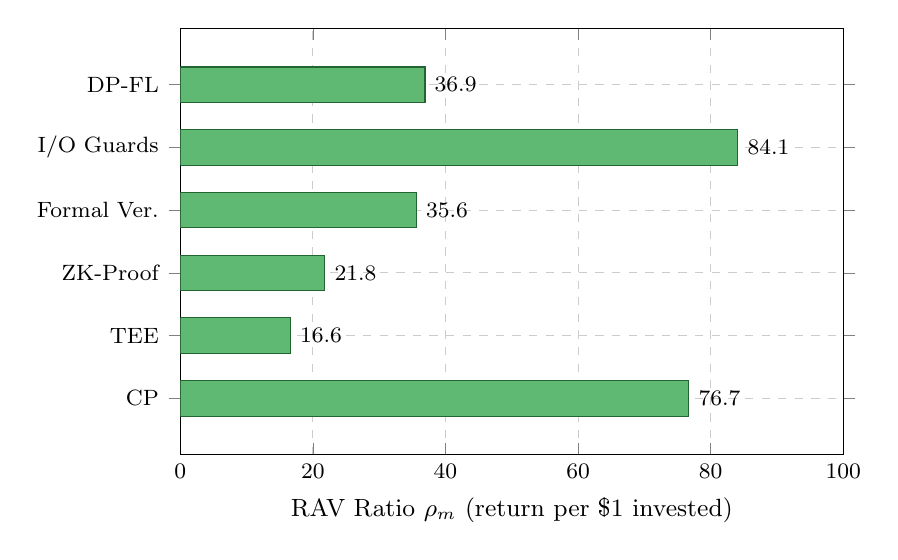
\begin{tikzpicture}
\begin{axis}[
    xbar,
    width=10cm, height=7cm,
    xlabel={RAV Ratio $\rho_m$ (return per \$1 invested)},
    symbolic y coords={CP,TEE,ZK-Proof,Formal Ver.,I/O Guards,DP-FL},
    ytick=data,
    xmin=0, xmax=100,
    nodes near coords,
    nodes near coords align={horizontal},
    nodes near coords style={font=\footnotesize},
    bar width=0.45cm,
    enlarge y limits=0.18,
    grid=major, grid style={dashed, gray!40},
    tick label style={font=\footnotesize},
    label style={font=\small},
  ]
  \addplot[fill=gaincol!80, draw=gaincol!60!black] coordinates {
    (76.7,CP)
    (16.6,TEE)
    (21.8,ZK-Proof)
    (35.6,Formal Ver.)
    (84.1,I/O Guards)
    (36.9,DP-FL)
  };
\end{axis}
\end{tikzpicture}
\caption{RAV Ratio $\rho_m$ for each trust mechanism in the
  Vietnamese fintech worked example.
  Input/Output Guardrails and Conformal Prediction deliver the
  highest return per dollar invested, making them the correct
  starting point for a constrained trust budget.
  ZK-Proofs and TEEs have lower ratios but defend against
  higher-severity incident classes and should be prioritised
  once the high-ratio mechanisms are in place.}
\label{fig:rav-prioritisation}
\end{figure}

% ------------------------------------------------------------------
\section{The CFO Conversation: A One-Page Summary Template}
\label{sec:cfo-summary}
% ------------------------------------------------------------------

The following template translates the RAV framework output
into the language a financial decision-maker requires.
Architects should populate this template with their
organisation-specific values before any budget discussion.

\begin{tcolorbox}[formulabox,
  title={One-Page RAV Summary Template}]

\textbf{Organisation:} \underline{\hspace{4cm}}
\quad
\textbf{Deployment:} \underline{\hspace{4cm}}
\quad
\textbf{Date:} \underline{\hspace{2cm}}

\medskip
\begin{tabular}{@{}p{5cm} r@{}}
Total annual loss exposure (unprotected) &
  \$ \underline{\hspace{2.5cm}} \\
Proposed trust mechanism stack &
  \underline{\hspace{2.5cm}} \\
Total annual mechanism cost $\sum C_{m_i}$ &
  \$ \underline{\hspace{2.5cm}} \\
Portfolio RAV $\mathrm{RAV}(M)$ &
  \$ \underline{\hspace{2.5cm}} \\
RAV Ratio $\rho = \mathrm{RAV}(M) / \sum C_{m_i}$ &
  \underline{\hspace{2.5cm}}$\times$ \\
Residual risk after stack $p_{\mathrm{residual}}^{(k)}$ &
  \underline{\hspace{2.5cm}}\% per year \\
Regulatory mandate driving investment &
  \underline{\hspace{2.5cm}} \\
\end{tabular}

\medskip
\textbf{The ask:}
Approve \$\underline{\hspace{1.5cm}} in annual trust mechanism
investment to reduce expected annual loss from
\$\underline{\hspace{1.5cm}} (unprotected) to
\$\underline{\hspace{1.5cm}} (protected), delivering a
\underline{\hspace{0.8cm}}$\times$ return on every dollar
invested in trust.

\medskip
\textbf{The regulatory floor:}
Under \underline{\hspace{2cm}} [Decree~13 / AI Law / EU AI Act],
non-compliance carries a mandatory minimum penalty of
\$\underline{\hspace{1.5cm}}, making the proposed investment
a legal requirement independent of the RAV calculation.
\end{tcolorbox}

% ------------------------------------------------------------------
\section{Limitations of the RAV Framework}
\label{sec:rav-limitations}
% ------------------------------------------------------------------

The RAV framework is a decision-support tool, not a precise
actuarial calculation.
Architects and executives should be aware of four structural
limitations:

\begin{enumerate}
  \item \textbf{Probability estimation is the dominant source
    of uncertainty.}
    The default probabilities of Table~\ref{tab:default-probabilities}
    are conservative starting points, not calibrated estimates.
    Organisations operating in higher-threat environments
    (e.g., those handling biometric data under active
    nation-state threat) should commission a formal threat
    intelligence assessment to replace these defaults.

  \item \textbf{The RAV formula assumes independence between
    incident classes.}
    In practice, a single breach event may trigger costs
    across multiple incident classes simultaneously
    (e.g., a prompt-injection attack that also exfiltrates
    training data triggers both PII breach and MIA costs).
    The Residual Risk Chain of
    Equation~\eqref{eq:residual-risk} partially addresses
    this for within-class stacking, but cross-class
    correlation requires a more sophisticated joint
    probability model beyond the scope of this appendix.

  \item \textbf{Reputational costs are the hardest to
    quantify and the most organisation-specific.}
    The financial autopsies of
    Section~\ref{sec:incident-taxonomy} include reputational
    damage estimates derived from industry benchmarks.
    For organisations where brand trust is a primary revenue
    driver (e.g., healthcare providers, public-sector AI
    deployments), these estimates may significantly
    understate the true reputational exposure.

  \item \textbf{The RAV framework does not capture the
    compounding value of trust reputation.}
    A system with a documented, audited Trustworthy AI Stack
    is not only lower-risk than an unprotected system ---
    it is also more likely to win enterprise contracts,
    satisfy procurement requirements, and attract regulatory
    goodwill.
    These positive externalities are real but are not
    captured in the RAV formula.
    Architects should cite them qualitatively alongside the
    quantitative RAV calculation.
\end{enumerate}

% ------------------------------------------------------------------
\section{Conclusion: Trust as a Financial Instrument}
\label{sec:app-conclusion}
% ------------------------------------------------------------------

The Risk-Adjusted Value framework reframes Trustworthy AI not
as a cost centre but as a \textbf{financial instrument}:
a structured investment that generates a quantifiable, positive
expected return by reducing the probability and magnitude of
catastrophic loss events.

The four financial autopsies of this appendix demonstrate that
the cost ratios between prevention and remediation range from
$47\times$ to over $900\times$ across the incident classes
of the 2025 crisis.
No rational financial decision-maker, presented with these
numbers and a credible probability estimate, would decline to
invest in prevention.

The architect's job, in the CFO meeting, is to provide exactly
that: a credible, structured, quantified case that translates
the technical language of zero-knowledge proofs and conformal
prediction into the financial language of expected loss,
risk reduction, and return on investment.

This appendix has provided the tools.
The conversation is yours to have.
